\documentclass{article}
\usepackage[utf8]{inputenc}
\usepackage[french]{babel}
\usepackage{amsmath}
\usepackage{amsfonts}
\usepackage{amssymb}
\usepackage{algorithm}
\usepackage{graphicx}
\usepackage[font=small, labelfont=bf]{caption}
\documentclass{report}
\usepackage[]{algpseudocode}

\title{
	Bomberman \\
	\large Rapport du projet de programmation impérative	
}
\date{\today}
\author{Quentin Januel & Clément Defrétière}

\begin{document}

\maketitle
\begin{abstract}
Pendant toute la réalisation du projet, les collisions ont été la plus importante difficulté à laquelle nous avons été confronté. Il nous semble donc pertinent de leur consacrer ce rapport. Il y aura donc de nombreux points que l'on se contentera de taire afin de garder ce document aussi concis que possible, cependant lire le code source suffit à assimiler ces derniers.
\newpage

Les collisions sont sources de beaucoup de problèmes dans les jeux vidéos. Dans le cadre de notre Bomberman, nous avions naïvement commencé par les coder de la façon suivante :
\begin{algorithm}
\begin{algorithmic}[1]
\State $nextPosition \gets \texttt{getNextPositionFromInputs}()$
\If {$\texttt{playerCollidesAt}(nextPosition)$}
\While{$\textbf{not} \texttt{playerCollidesAt}(\texttt{onePixelToward}(nextPosition))$}
\State $\texttt{movePlayerTo}(\texttt{onePixelToward}(nextPosition))$
\EndWhile
\Else
\State $\texttt{movePlayerTo}(nextPosition)$
\EndIf
\end{algorithmic}
\end{algorithm}

C'est-à-dire que le programme empêchait formellement au joueur d'être en collision avec un obstacle : on vérifie d'abord s'il y a un obstacle là où le joueur est censé se rendre, si non, il peut bouger, si oui on le fait bouger dans cette direction pixel par pixel tant qu'aucune collision ne pose problème. \\
Pour être plus précis, notre code séparait ce pseudo-code en deux parties : le movement horizontal et celui vertical, de sorte qu'il n'y ait pas de trigonométrie impliquée. \\

Le joueur a une vitesse $x$ et bouge donc de $x$ pixels par frame. De plus, la hitbox du joueur est un carré de $n \times n$ pixels et ce dernier se déplace dans des couloirs ayant exactement ses dimensions, ce qui produit le problème suivant : \\
\begin{center}
\begin{tabular}{cc}
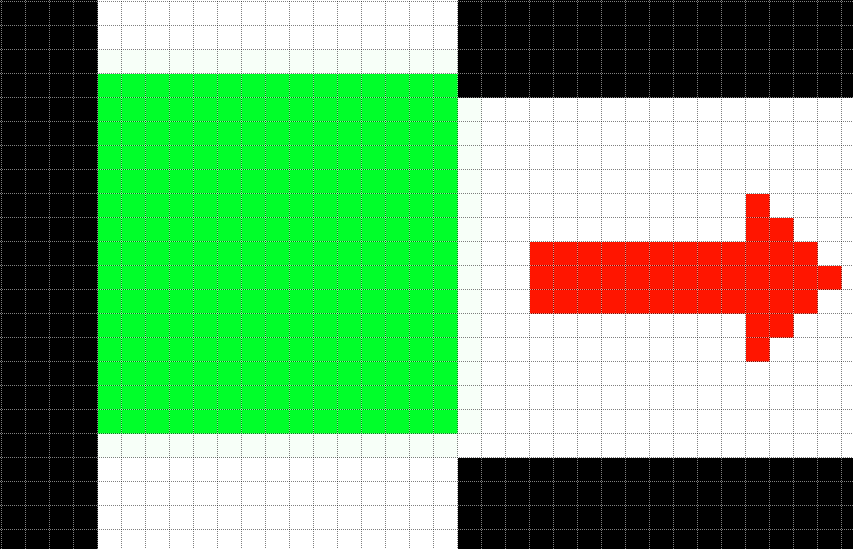
\includegraphics[scale=0.2]{fig1.png} &
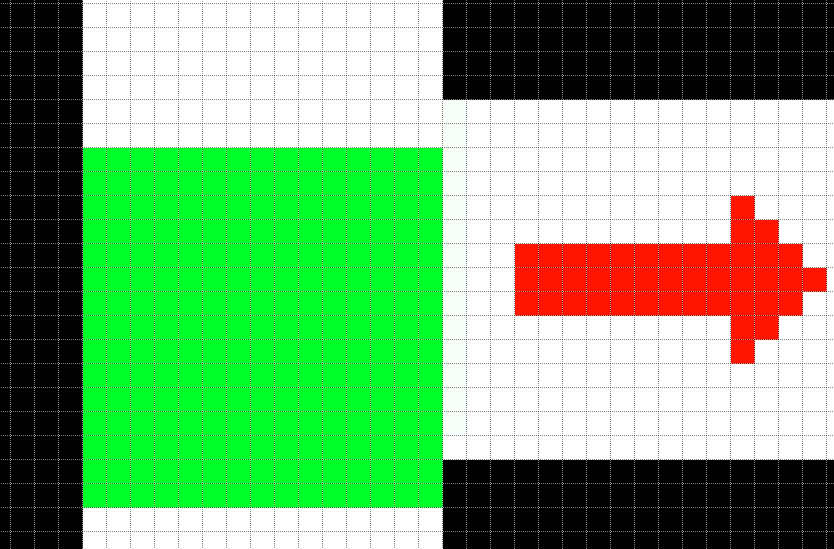
\includegraphics[scale=0.2]{fig2.png} \\
\textbf{Fig. 1} & \textbf{Fig. 2} \\
\end{tabular}
\end{center}
Le joueur (le carré vert) se trouve en \textbf{Fig. 1} et cherche à rentrer dans le couloir indiqué par la flèche rouge. Il lui est impossible d'aller à droite car il serait alors en collision avec l'obstacle noir et le programme interdit ça. Cependant, s'il descend pendant une frame, sa coordonnée verticale augmente de $x = 3$ pixels (voir \textbf{Fig. 2}) ce qui ne lui permet toujours pas de rentrer dans le couloir. Le joueur ne pourra donc jamais y accéder. Pour y remédier, nous avons imaginé deux astuces. \\

La première consiste à ne pas bouger de $x$ pixels par frame mais de seulement $1$. Ensuite, répéter la procédure $x$ fois par frame. Au final, le joueur aura bien bougé de $x$ pixels mais ce en $x$ fois et comme les inputs ne sont récupérés qu'une fois par frame, le jeu laissera passer le joueur dans le couloir si ce dernier appuie sur droite et bas en même temps depuis \textbf{Fig. 1}. \\

La seconde est un tout autre algorithme de collision :
\begin{algorithm}
\begin{algorithmic}[1]
\State $tempPosition \gets \texttt{getNextPositionFromInputs}()$
\State $\texttt{movePlayerTo}(tempPosition)$
\If {$\texttt{playerIsColliding}()$}
\State $minDistance \gets +\infty$
\State $angleOfMinDistance \gets 0$
\For{$angle = 0; angle < 360; angle \gets angle+45$}
\State $currentDistance \gets 0$
\While {$\texttt{playerIsColliding}()$}
\State $newPosition \gets tempPosition + \texttt{vector}(1, angle))$
\State $\texttt{movePlayerTo}(newPosition)$
\State $currentDistance \gets currentDistance+1$
\EndWhile
\If {$currentDistance < minDistance$}
\State $minDistance \gets currentDistance$
\State $angleOfMinDistance \gets angle$
\EndIf
\State $\texttt{movePlayerTo}(tempPosition)$
\EndFor
\State $newPosition \gets tempPosition + \texttt{vector}(minDistance, angleOfMinDistance))$
\State $\texttt{movePlayerTo}(newPosition)$
\EndIf
\end{algorithmic}
\end{algorithm}

Le principe est de laisser le joueur se déplacer, et seulement ensuite le faire sortir de l'obstacle en le poussant dans la direction la moins couteuse en distance.
Cependant, l'algorithme tel quel ne convient pas : en effet si le joueur se trouve sous un obstacle et tente de monter (voir \textbf{Fig. 3 \& 4}), le jeu le repoussera dans la meilleure direction. Mais il n'y a aucune différence entre le pousser dans la direction bas-gauche, bas tout court et bas-droite. Si l'on décide de redéfinir la distance minimale seulement si l'on a trouvé une distance strictement plus court, alors c'est la première calculée (bas-gauche) qui sera prise en compte. Et si on laisse l'inégalité non stricte, alors c'est la dernière calculée (bas-droite) qui sera prise en compte.
Au final, dans les deux cas, si le joueur monte alors qu'un obstacle l'en empêche, alors il observera son personnage se déplacer latéralement (voir \textbf{Fig. 5}). \\
\begin{center}
\begin{tabular}{ccc}
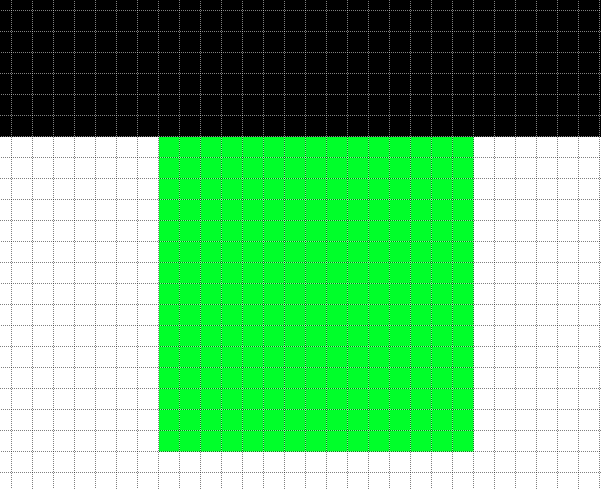
\includegraphics[scale=0.2]{fig3.png} &
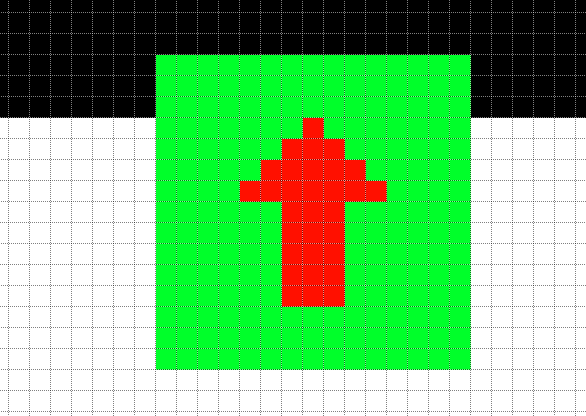
\includegraphics[scale=0.2]{fig4.png} &
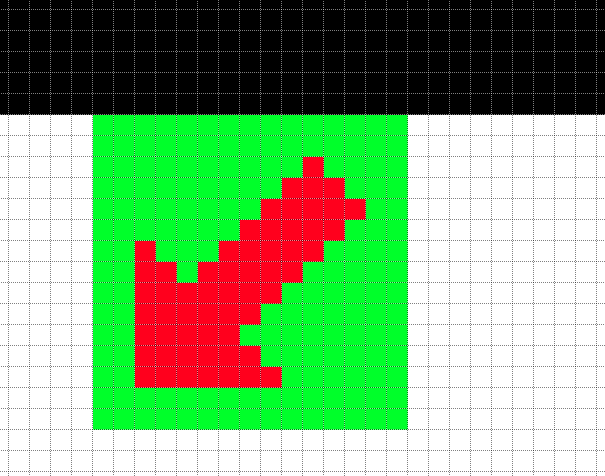
\includegraphics[scale=0.2]{fig5.png} \\
\textbf{Fig. 3} & \textbf{Fig. 4} & \textbf{Fig. 5} \\
\end{tabular}
\end{center}
Pour y remédier, on pourrait d'abord penser à supprimer les directions diagonales de l'algorithme mais ce serait retirer un bug pour en rajouter un autre :
Si le joueur se trouve en \textbf{Fig. 6} et bouge en diagonale direction haut-gauche (\textbf{Fig. 7}), alors le jeu, incapable de le renvoyer d'où il vient sans diagonales,² le repoussera comme indiqué sur \textbf{Fig. 8}. \\
\begin{center}
\begin{tabular}{ccc}
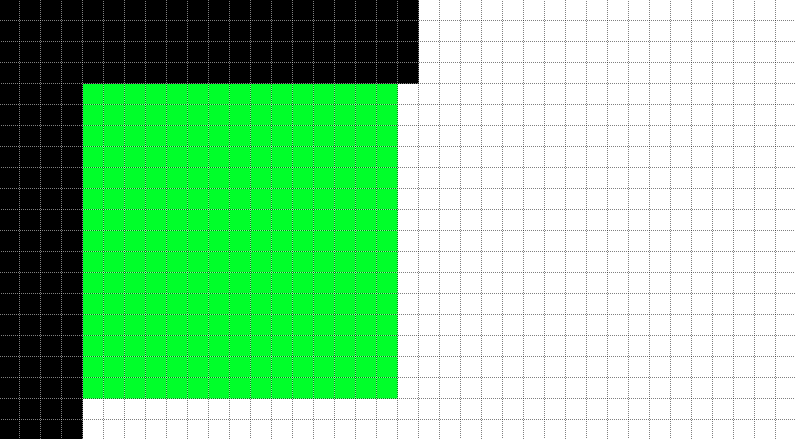
\includegraphics[scale=0.2]{fig6.png} &
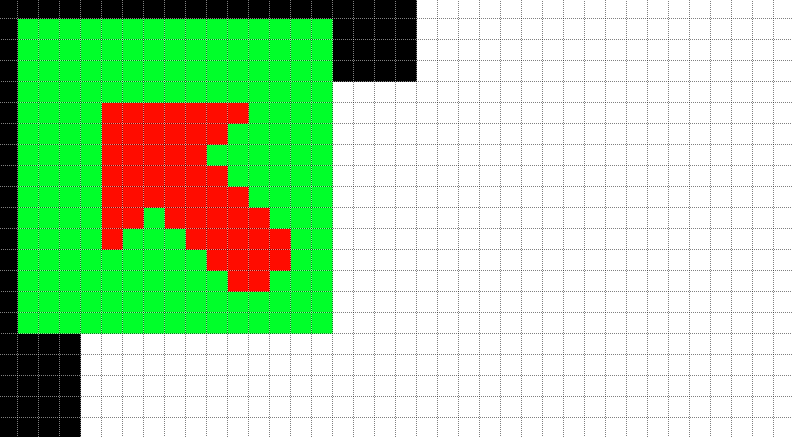
\includegraphics[scale=0.2]{fig7.png} &
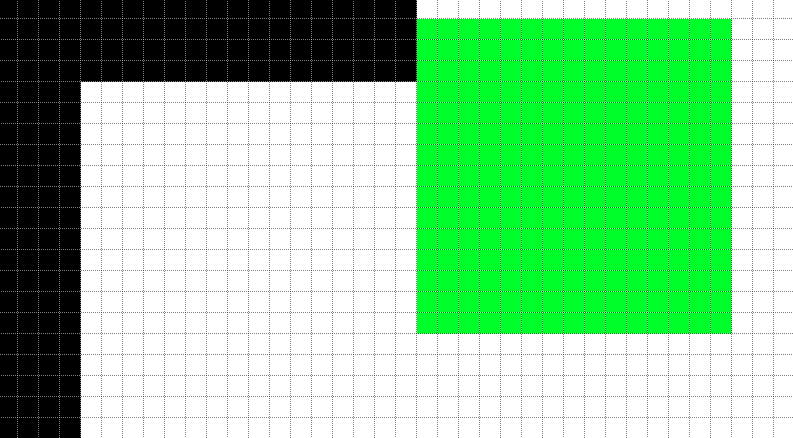
\includegraphics[scale=0.2]{fig8.png} \\
\textbf{Fig. 6} & \textbf{Fig. 7} & \textbf{Fig. 8} \\
\end{tabular}
\end{center}
On a alors simplement redéfini la distance minimale uniquement si une distance $d$ est strictement plus courte, ou autant bonne mais non diagonale. \\

Il s'agit maintenant de choisir entre les deux solutions à notre disposition.
Une analyse de complexité ne semble pas pertinente car, en supposant que playerIsColliding et playerCollidesAt soient $O(1)$ ce qui n'est pas le cas mais qui ne change rien, les deux solutions sont linéaires ($O(x)$ avec $x$ la vitesse du joueur).
Toutefois, même si la solution deux multiplie le nombre d'itérations par $8$ (= nombre de directions), elle ne se produit que lorsque le joueur est en collision tandis que la solution 1 se trouve dans le pire cas à chaque frame. C'est pourquoi nous avons choisi la deuxième solution.
Il y a possiblement des bugs que possède la première solution mais ne l'ayant pas implémentée nous n'avons pas eu l'occasion de les rencontrer.
\newpage

\end{document}
